\documentclass[10pt,letterpaper]{article}
\usepackage[utf8]{inputenc}
\usepackage[T1]{fontenc}
\usepackage[margin=0.6in]{geometry}
\usepackage{amsmath,amssymb,mathtools,graphicx,booktabs,xcolor,hyperref}
\setlength{\parindent}{0pt}
\setlength{\parskip}{5pt}
\begin{document}

{\color{ink}\sffamily\bfseries\LARGE Block S1 Solutions: Equivalent Resistance \& Multi-Source KVL/KCL}\par
\textbf{Companion Key to:} \texttt{Block\_S1\_Exercises\_EqResistance\_KVL\_KCL.pdf} \quad|\quad \textbf{MNA Solver Check:} All nodal voltages \& branch currents verified

\section*{Exercise 01 Solutions $\cdot$ First-Principles \& Conical Conductor Calculus Proof \hfill [10 Points]}
\textbf{(a) Series Equivalent Resistance [2 pts]:} In steady state ($\nabla\cdot\mathbf{J}=0$), KCL at each internal junction ensures identical current $I_1 = I_2 = \dots = I_N = I$. Applying KVL ($\sum_{\rm loop}\Delta V=0$), including the source rise, around the loop:
\[
  V_{ab} - \sum_{k=1}^N I R_k = 0 \implies V_{ab} = I \sum_{k=1}^N R_k \implies R_{\text{eq}} = \frac{V_{ab}}{I} = \sum_{k=1}^N R_k. \quad \blacksquare
\]
\textbf{(b) Parallel Equivalent Resistance \& Upper Bound [2 pts]:} The same two nodes enforce identical branch voltage $V_k = V_{ab}$. Applying KCL at node $a$ for $N\ge2$ positive resistors:
\[
  I_{\text{total}} = \sum_{k=1}^N I_k = V_{ab}\sum_{k=1}^N \frac{1}{R_k} \implies \frac{1}{R_{\text{eq}}} = \sum_{k=1}^N \frac{1}{R_k} = \frac{1}{R_{\min}} + \sum_{k\neq\min}\frac{1}{R_k} > \frac{1}{R_{\min}} \implies R_{\text{eq}} < R_{\min}. \quad \blacksquare
\]
\textbf{(c) Continuous Tapered Conical Conductor [6 pts]:} These results are exact within the stated one-dimensional equipotential-slice model; a physical tapered conductor can have spreading fields.
\begin{enumerate}
  \item[(i)] $r(x) = a + \frac{b-a}{L}x$, \quad $A(x) = \pi\left[a + \frac{b-a}{L}x\right]^2$, \quad $dR = \dfrac{\rho\,dx}{\pi\left[a + \frac{b-a}{L}x\right]^2}$.
  \item[(ii)] With $u = a + \frac{b-a}{L}x$ and $dx = \frac{L}{b-a}\,du$:
  \[
    R = \frac{\rho L}{\pi(b-a)}\int_a^b u^{-2}\,du = \frac{\rho L}{\pi(b-a)}\left(\frac{1}{a}-\frac{1}{b}\right) = \frac{\rho L}{\pi a b}.
  \]
  \item[(iii)] As $b \to a$, $R \to \frac{\rho L}{\pi a^2} = \frac{\rho L}{A}$. Inside the frustum, $E(x) = \rho J(x) = \dfrac{\rho I}{\pi[a + (b-a)x/L]^2}$.
\end{enumerate}

\section*{Exercise 02 Solutions $\cdot$ Mixed Series--Parallel DC Ladder \hfill [10 Points]}
\begin{enumerate}
  \item[(a)] $R_{34} = R_3 + R_4 = 4.00 + 5.00 = 9.00\ \Omega$; \quad $R_{BG} = \frac{(18.0)(9.00)}{18.0+9.00} = 6.00\ \Omega$; \quad $R_{\text{eq}} = R_1 + R_{BG} = 6.00 + 6.00 = 12.0\ \Omega$.
  \item[(b)] $I_{\text{src}} = \frac{36.0}{12.0} = 3.00\text{ A}$; \quad $V_B = 36.0 - (3.00)(6.00) = 18.0\text{ V}$; \quad $I_2 = \frac{18.0}{18.0} = 1.00\text{ A}$; \quad $I_{34} = \frac{18.0}{9.00} = 2.00\text{ A}$; \quad $V_D = I_{34}R_4 = 10.0\text{ V}$.
  \item[(c)] $P_{R_1}=54.0\text{ W}$, $P_{R_2}=18.0\text{ W}$, $P_{R_3}=16.0\text{ W}$, $P_{R_4}=20.0\text{ W}$; \quad $\sum P_{R_k} = 108.0\text{ W} = (36.0\text{ V})(3.00\text{ A})$.
  \item[(d)] Shorting $R_3 \to 0$: $R_{BG}' = \frac{(18.0)(5.00)}{23.0} = \frac{90}{23}\ \Omega \approx 3.913\ \Omega$, \quad $R_{\text{eq}}' = \frac{228}{23} \approx 9.91\ \Omega$, \quad $I_{\text{src}}' = \frac{69}{19} \approx 3.63\text{ A}$, \quad $V_B' = \frac{270}{19} \approx 14.21\text{ V}$, \quad $P_{R_4}' = \frac{(V_B')^2}{5.00} \approx 40.4\text{ W}$ ($2.02\times$ increase).
\end{enumerate}

\section*{Exercise 03 Solutions $\cdot$ Multi-Source KVL/KCL Network \hfill [12 Points]}
\begin{enumerate}
  \item[(a)] KCL at $A$: $I_1 + I_2 + I_3 = 0$. Left mesh KVL: $+18.0 + 3.00 I_1 - 6.00 I_2 = 0$. Right mesh KVL: $+6.00 I_2 - 3.00 I_3 - 9.00 = 0$.
  \item[(b)] Nodal KCL: $\frac{V_A - 18.0}{3.00} + \frac{V_A}{6.00} + \frac{V_A - 9.00}{3.00} = 0 \implies 5V_A = 54.0 \implies V_A = 10.8\text{ V}$. Thus $I_1 = -2.40\text{ A}$ ($2.40\text{ A}$ upward), $I_2 = +1.80\text{ A}$ (downward), $I_3 = +0.600\text{ A}$ (downward).
  \item[(c)] $\mathcal{E}_1$ delivers $P_{\mathcal{E}_1} = (18.0)(2.40) = 43.2\text{ W}$. $\mathcal{E}_3$ absorbs $P_{\mathcal{E}_3} = (9.00)(0.600) = 5.40\text{ W}$. Net delivered $= 37.8\text{ W} = 17.28 + 19.44 + 1.08 = \sum I_k^2 R_k$.
\end{enumerate}

\section*{Exercise 04 Solutions $\cdot$ Cloze \& Maximum Power Transfer \hfill [10 Points]}
\textbf{Part A Key:} (a) \texttt{electric charge}, (b) \texttt{energy}, (c) \texttt{smaller than}, (d) \texttt{opposite to}, (e) $\mathcal{E}-Ir$, (f) $\mathcal{E}+Ir$, (g) \texttt{open circuit}, (h) \texttt{short circuit}.\par
\textbf{Part B Proof:} $P_L(R_L) = \frac{\mathcal{E}^2 R_L}{(r+R_L)^2} \implies \frac{dP_L}{dR_L} = \mathcal{E}^2\frac{r-R_L}{(r+R_L)^3} = 0 \implies R_L = r = 3.00\ \Omega$, $P_{L,\max} = \frac{\mathcal{E}^2}{4r} = 27.0\text{ W}$.
\begin{center}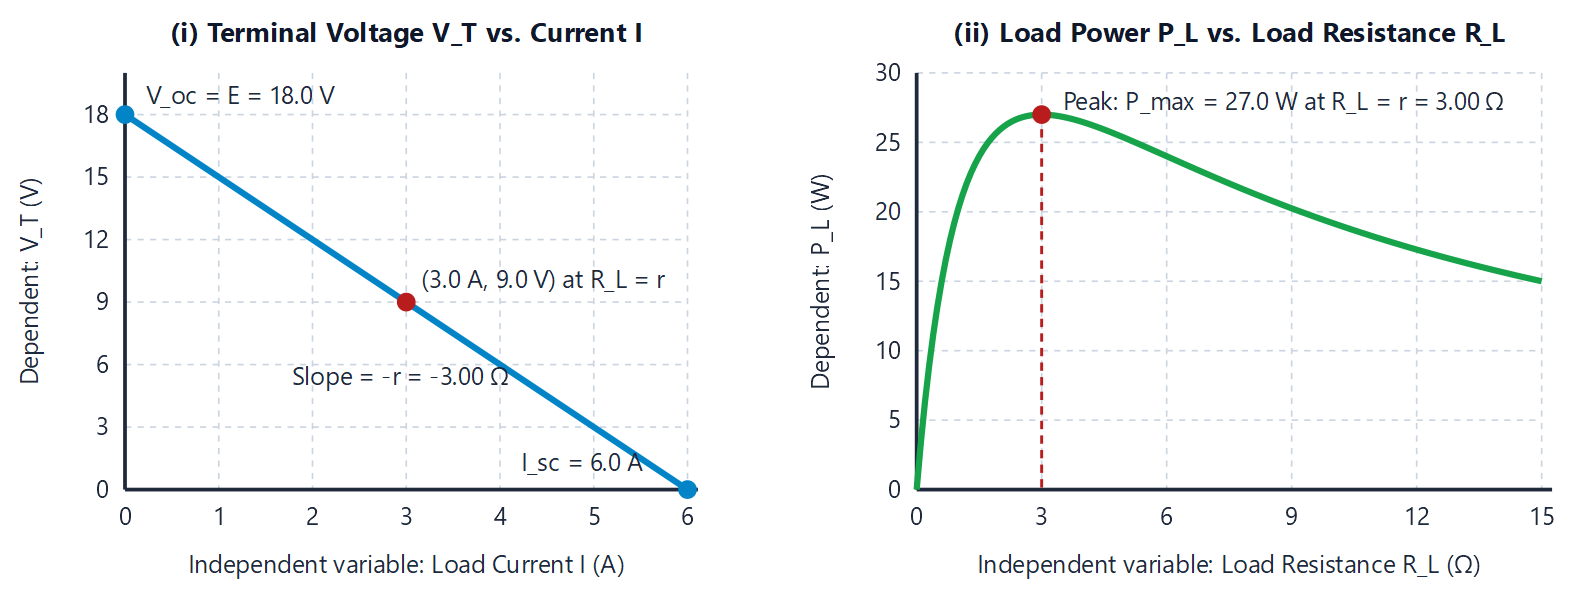
\includegraphics[width=0.92\linewidth]{block_s1_assets/s1-q4-grid-solved.png}\end{center}
\newpage
\section*{Block S2 Solutions: Wheatstone Bridge Analysis via KVL/KCL}

  \textbf{Companion Key to:} \texttt{Block\_S2\_Exercises\_Wheatstone\_Bridge.pdf} ~|~
  \textbf{Verification:} Cross-checked via Spec v2 Modified Nodal Analysis (MNA)


\subsection*{01 $\cdot$ Solutions: Null-Balance Condition \& Sensitivity Calculus Proof \hfill [10 Points]}


  \subsubsection*{(a) Null-Balance Proof from KCL \& KVL [4 points]}
  \textbf{(i) Node Potentials \& Leg Currents:} When $I_{LR} = 0$, Ohm's law across $R_G$ gives $V_L - V_R = I_{LR} R_G = 0 \implies V_L = V_R$. By KCL at node $L$, $I_1 = I_2 + I_{LR} = I_2$; by KCL at node $R$, $I_3 + I_{LR} = I_4 \implies I_3 = I_4$.
  \textbf{(ii) Ratio Proof:} Since $V_L = V_R$ and $V_B = 0\text{ V}$, the voltage drops across the upper resistors are equal ($V_T - V_L = V_T - V_R \implies I_1 R_1 = I_3 R_3$) and the voltage drops across the lower resistors are equal ($V_L = V_R \implies I_2 R_2 = I_4 R_4$). Dividing the first equation by the second and using $I_1 = I_2$, $I_3 = I_4$:
  $$\frac{I_1 R_1}{I_2 R_2} = \frac{I_3 R_3}{I_4 R_4} \implies \frac{R_1}{R_2} = \frac{R_3}{R_4} \Longleftrightarrow R_1 R_4 = R_2 R_3. \quad \blacksquare$$
  \textbf{(iii) Source \& Meter Independence:} Neither $V_T$ nor $R_G$ appears in $R_4 = \frac{R_2 R_3}{R_1}$ because both legs scale proportionally with $V_T$ ($V_L = \frac{R_2}{R_1+R_2}V_T$ and $V_R = \frac{R_4}{R_3+R_4}V_T$), so setting $V_L = V_R$ cancels $V_T$ completely (for any $V_T \neq 0$) and produces zero drop across any $R_G$.

  \subsubsection*{(b) Exact Unbalanced Bridge Current $I_{LR}(R_4)$ \& Sensitivity Derivative [6 points]}
  \textbf{(i) Closed-Form Formula [4 pts]:} Looking into node $L$ (with $R_G$ removed), the left voltage divider ($R_1 = 150\ \Omega, R_2 = 300\ \Omega$) has open-circuit voltage and Th\'evenin resistance:
  $$V_{\text{Th},L} = 15.0\left(\frac{300}{150 + 300}\right) = 10.0\text{ V}, \qquad R_{\text{Th},L} = \frac{(150)(300)}{150 + 300} = 100\ \Omega.$$
  Looking into node $R$, the right divider ($R_3 = 150\ \Omega$, variable $R_4$) has:
  $$V_{\text{Th},R}(R_4) = \frac{15.0 R_4}{150 + R_4}, \qquad R_{\text{Th},R}(R_4) = \frac{150 R_4}{150 + R_4}.$$
  Connecting $R_G = 100\ \Omega$ between $L$ and $R$ gives:
  $$I_{LR}(R_4) = \frac{V_{\text{Th},L} - V_{\text{Th},R}(R_4)}{R_{\text{Th},L} + R_G + R_{\text{Th},R}(R_4)} = \frac{10.0 - \frac{15.0 R_4}{150 + R_4}}{200 + \frac{150 R_4}{150 + R_4}} = \frac{1500 - 5.0 R_4}{30000 + 350 R_4} = \frac{300 - R_4}{6000 + 70 R_4}\text{ A} = \frac{300 - R_4}{6.00 + 0.0700 R_4}\text{ mA}.$$
  \textbf{(ii) Calculus Sensitivity at Balance [2 pts]:} Differentiating via the quotient rule:
  $$\frac{dI_{LR}}{dR_4} = \frac{(-1)(6000 + 70 R_4) - (300 - R_4)(70)}{(6000 + 70 R_4)^2} = \frac{-27000}{(6000 + 70 R_4)^2}\text{ A}/\Omega.$$
  Evaluating at $R_4 = 300\ \Omega$ ($6000 + 70(300) = 27000\ \Omega$):
  $$\left.\frac{dI_{LR}}{dR_4}\right|_{R_4 = 300\ \Omega} = -\frac{27000}{(27000)^2} = -\frac{1}{27000}\text{ A}/\Omega \approx -37.0\ \mu\text{A}/\Omega.$$

Final Key (Ex 01): ~ (a) $R_1/R_2 = R_3/R_4$ ~|~ (b) $I_{LR}(R_4) = \dfrac{300 - R_4}{6.00 + 0.0700 R_4}\text{ mA}$, ~ $\left.\dfrac{dI_{LR}}{dR_4}\right|_{300\ \Omega} = -37.0\ \mu\text{A}/\Omega$


\newpage



\subsection*{02 $\cdot$ Solutions: Unbalanced Wheatstone Bridge Nodal \& Mesh Analysis \hfill [14 Points]}


  \textbf{(a) Irreducibility [2 pts]:} Because node $L$ is a 3-way junction connecting $R_1, R_2$, and $R_G$ (with $I_{LR} \neq 0$), $R_1$ and $R_2$ do not carry the same current (not in series), and $R_1$ and $R_3$ do not share both terminal nodes because $R_G$ separates $L$ from $R$ (not in parallel).
  \textbf{(b) KCL \& KVL Equations [4 pts]:} With $V_T = 15.0\text{ V}$ and $V_B = 0\text{ V}$:
  \begin{itemize}
    \item \textbf{KCL at node $L$:} $\dfrac{V_L - 15.0}{150} + \dfrac{V_L - 0}{300} + \dfrac{V_L - V_R}{100} = 0 \xrightarrow{\times 300} 2(V_L - 15.0) + V_L + 3(V_L - V_R) = 0 \implies 6 V_L - 3 V_R = 30.0 \implies 2 V_L - V_R = 10.0$.
    \item \textbf{KCL at node $R$:} $\dfrac{V_R - 15.0}{150} + \dfrac{V_R - 0}{150} + \dfrac{V_R - V_L}{100} = 0 \xrightarrow{\times 300} 2(V_R - 15.0) + 2 V_R + 3(V_R - V_L) = 0 \implies -3 V_L + 7 V_R = 30.0$.
    \item \textbf{KVL around upper loop ($T \to L \to R \to T$):} $-150 I_1 - 100 I_{LR} + 150 I_3 = 0$.
  \end{itemize}
  \textbf{(c) Solving for $V_L, V_R$, and $I_{LR}$ [5 pts]:} From the first equation, $V_R = 2 V_L - 10.0$. Substituting into the second equation:
  $$-3 V_L + 7(2 V_L - 10.0) = 30.0 \implies 11 V_L = 100.0 \implies V_L = \frac{100}{11}\text{ V} \approx 9.09\text{ V}, \qquad V_R = \frac{90}{11}\text{ V} \approx 8.18\text{ V}.$$
  The signed bridge current from $L$ to $R$ is:
  $$I_{LR} = \frac{V_L - V_R}{R_G} = \frac{10/11\text{ V}}{100\ \Omega} = +\frac{1}{110}\text{ A} \approx +9.09\text{ mA}\text{ (flows from }L\text{ to }R\text{)}.$$
  \textbf{(d) All Leg Currents \& $R_{\text{eq}}$ [3 pts]:}
  $$I_1 = \frac{15 - 100/11}{150} = \frac{65/11}{150} = \frac{13}{330}\text{ A} \approx 39.4\text{ mA}, \qquad I_2 = \frac{100/11}{300} = \frac{1}{33}\text{ A} \approx 30.3\text{ mA},$$
  $$I_3 = \frac{15 - 90/11}{150} = \frac{75/11}{150} = \frac{1}{22}\text{ A} \approx 45.5\text{ mA}, \qquad I_4 = \frac{90/11}{150} = \frac{3}{55}\text{ A} \approx 54.5\text{ mA}.$$
  $$I_{\text{src}} = I_1 + I_3 = \frac{13}{330} + \frac{15}{330} = \frac{28}{330} = \frac{14}{165}\text{ A} \approx 84.8\text{ mA}, \qquad R_{\text{eq}} = \frac{15.0\text{ V}}{14/165\text{ A}} = \frac{2475}{14}\ \Omega \approx 177\ \Omega.$$

Final Key (Ex 02): ~ $V_L = 9.09\text{ V},\ V_R = 8.18\text{ V}$ ~|~ $I_{LR} = +9.09\text{ mA}$ ($L \to R$) ~|~ $I_{\text{src}} = 84.8\text{ mA},\ R_{\text{eq}} = 177\ \Omega$

\subsection*{03 $\cdot$ Solutions: Bridge Current Curve $I_{LR}(R_4)$ \& Conceptual Cloze \hfill [10 Points]}


  \textbf{Part A Landmark Values:} (1) $I_{LR}(0) = +50.0\text{ mA}$; (2) $I_{LR}(150\ \Omega) = +9.09\text{ mA}$; (3) $I_{LR}(300\ \Omega) = 0\text{ mA}$ (balanced); (4) $\lim_{R_4\to\infty} I_{LR}(R_4) = -\frac{1}{0.0700} = -14.3\text{ mA}$.
  \textbf{Part B Cloze Key:} (a) \texttt{zero}, \texttt{equal to}; (b) \texttt{$300\ \Omega$}; (c) \texttt{from $L$ to $R$}; (d) \texttt{from $R$ to $L$}; (e) \texttt{unchanged}; (f) \texttt{both an open and a short circuit}; (g) \texttt{Kirchhoff's junction rule}.

\begin{center}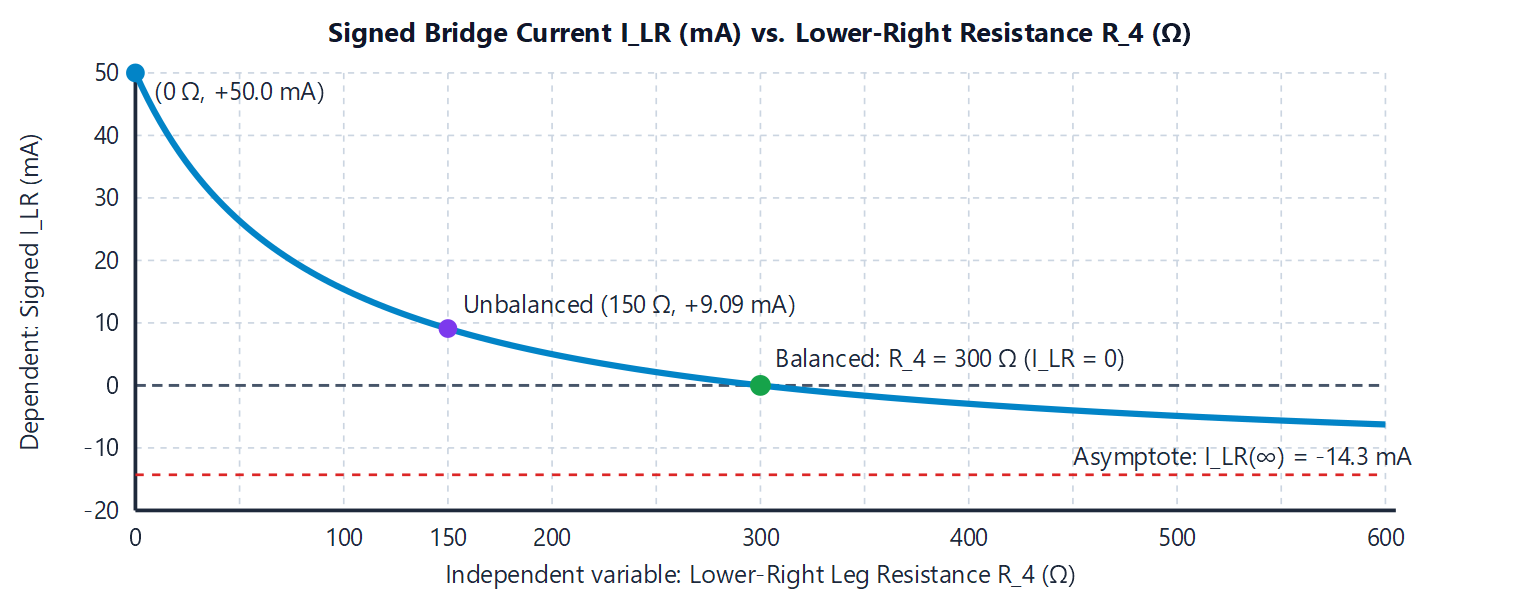
\includegraphics[width=0.82\linewidth]{day1_assets/s2-q3-grid-solved.png}\end{center}
\newpage
\section*{Block S3 Solutions: RC Charging \& Discharging Transients}

  \textbf{Companion Key to:} \texttt{Block\_S3\_Exercises\_RC\_Transients.pdf} ~|~
  \textbf{Verification:} ODE \& Energy Integrals Verified Analytically \& Numerically


\subsection*{01 $\cdot$ Solutions: First-Order RC ODE \& Separation of Variables \hfill [10 Points]}


  \subsubsection*{(a) Charging ODE \& Separation of Variables [6 points]}
  \textbf{(i) KVL Differential Equation [2 pts]:} Traversing the loop in the direction of $i(t) = \frac{dq}{dt}$:
  $$\mathcal{E} - iR - \frac{q}{C} = 0 \implies R\frac{dq}{dt} + \frac{q}{C} = \mathcal{E} \implies \frac{dq}{dt} = \frac{C\mathcal{E} - q}{RC}.$$
  \textbf{(ii) Definite Integration [4 pts]:} Separating $q'$ and $t'$ and integrating from $(0,0)$ to $(t, q(t))$:
  $$\int_{0}^{q(t)} \frac{dq'}{C\mathcal{E} - q'} = \int_{0}^{t} \frac{dt'}{RC} \implies \Big[-\ln(C\mathcal{E} - q')\Big]_{0}^{q(t)} = \frac{t}{RC} \implies \ln\left(\frac{C\mathcal{E} - q(t)}{C\mathcal{E}}\right) = -\frac{t}{RC}.$$
  Exponentiating both sides with $\tau = RC$:
  $$1 - \frac{q(t)}{C\mathcal{E}} = e^{-t/\tau} \implies q(t) = C\mathcal{E}\left(1 - e^{-t/(RC)}\right), \quad v_C(t) = \frac{q(t)}{C} = \mathcal{E}\left(1 - e^{-t/(RC)}\right), \quad i(t) = \frac{dq}{dt} = \frac{\mathcal{E}}{R}e^{-t/(RC)}. \quad \blacksquare$$

  \subsubsection*{(b) Discharging from Initial Charge $Q_0 = C V_{\text{init}}$ [4 points]}
  With no battery in the loop, KVL gives $R\frac{dq}{dt} + \frac{q}{C} = 0$. Separating variables:
  $$\int_{Q_0}^{q(t)} \frac{dq'}{q'} = -\int_{0}^{t} \frac{dt'}{RC} \implies \ln\left(\frac{q(t)}{Q_0}\right) = -\frac{t}{RC} \implies q(t) = Q_0 e^{-t/(RC)}, \quad v_C(t) = V_{\text{init}} e^{-t/(RC)}. \quad \blacksquare$$


\subsection*{02 $\cdot$ Solutions: Calculus Proof of Half-Energy Dissipation \hfill [10 Points]}


  \textbf{(a) Total Charge \& Battery Work [3 pts]:}
  $$Q_{\text{final}} = \int_{0}^{\infty} \frac{\mathcal{E}}{R}e^{-t/(RC)}\,dt = \frac{\mathcal{E}}{R}\Big[-RC e^{-t/(RC)}\Big]_{0}^{\infty} = C\mathcal{E}, \qquad W_{\text{batt}} = \mathcal{E} Q_{\text{final}} = C\mathcal{E}^2.$$
  \textbf{(b) Resistor Joule Heating Integral [5 pts]:}
  $$E_{\text{dissipated}} = \int_{0}^{\infty} [i(t)]^2 R\,dt = \int_{0}^{\infty} \frac{\mathcal{E}^2}{R^2} e^{-2t/(RC)} R\,dt = \frac{\mathcal{E}^2}{R} \left[-\frac{RC}{2} e^{-2t/(RC)}\right]_{0}^{\infty} = \frac{\mathcal{E}^2}{R}\left(\frac{RC}{2}\right) = \frac{1}{2}C\mathcal{E}^2. \quad \blacksquare$$
  \textbf{(c) Energy Accounting \& Independence from $R$ [2 pts]:} The capacitor stores $U_C = \frac{1}{2}C\mathcal{E}^2$, so $U_C + E_{\text{dissipated}} = \frac{1}{2}C\mathcal{E}^2 + \frac{1}{2}C\mathcal{E}^2 = C\mathcal{E}^2 = W_{\text{batt}}$ (exact 50\%/50\% split!). If $R$ is halved, the initial power $P_R(0) = \mathcal{E}^2/R$ doubles, but the decay time constant $\tau = RC$ is halved, so the area under $P_R(t)$ remains invariant at $\frac{1}{2}C\mathcal{E}^2$.

Final Key (Ex 01 \& 02): ~ $q(t) = C\mathcal{E}(1 - e^{-t/RC})$ ~|~ $W_{\text{batt}} = C\mathcal{E}^2$ ~|~ $E_{\text{dissipated}} = \int_0^\infty i^2 R\,dt = \frac{1}{2}C\mathcal{E}^2 = U_C$


\newpage



\subsection*{03 $\cdot$ Solutions: Two-Position Switch RC Transient Analysis \hfill [10 Points]}


  \textbf{(a) Time Constant \& $t = 0^+$ State [2 pts]:}
  $$\tau = RC = (50.0\times 10^3\ \Omega)(20.0\times 10^{-6}\text{ F}) = 1.00\text{ s}, \qquad v_C(0^+) = v_C(0^-) = 0\text{ V}, \qquad i(0^+) = \frac{V_0 - 0}{R} = \frac{15.0\text{ V}}{50.0\text{ k}\Omega} = +300\ \mu\text{A}.$$
  \textbf{(b) State Just Before Switching ($t_1^- = 2.00\text{ s}^-$) [3 pts]:} On $0 \le t < 2.00\text{ s}$, $v_C(t) = 15.0(1 - e^{-t/1.00})\text{ V}$ and $i(t) = 300 e^{-t/1.00}\ \mu\text{A}$:
  $$v_C(2.00\text{ s}^-) = 15.0\left(1 - e^{-2.00}\right) = 15.0(1 - 0.13534) = 12.97\text{ V} \approx 13.0\text{ V},$$
  $$i(2.00\text{ s}^-) = 300 e^{-2.00}\ \mu\text{A} = 300(0.13534) = +40.6\ \mu\text{A}.$$
  \textbf{(c) Switching Instant Continuity \& Jump ($t_1^+ = 2.00\text{ s}^+$) [3 pts]:}
  \begin{itemize}
    \item \textbf{Voltage Continuity:} $v_C(2.00\text{ s}^+) = v_C(2.00\text{ s}^-) = 12.97\text{ V}$ because a step jump $\Delta v_C \neq 0$ in zero time $\Delta t \to 0$ would require infinite current $i = C\frac{dv_C}{dt} \to \infty$, which is impossible through finite resistance $R = 50.0\text{ k}\Omega$.
    \item \textbf{Current Jump:} At $t_1^+ = 2.00\text{ s}^+$, the left side of $R$ is grounded ($0\text{ V}$) while the right side (Node $B$) is at $+12.97\text{ V}$:
    $$i(2.00\text{ s}^+) = \frac{0 - v_C(2.00\text{ s}^+)}{R} = -\frac{12.97\text{ V}}{50.0\text{ k}\Omega} = -259.4\ \mu\text{A} \approx -259\ \mu\text{A}.$$
    The jump is $\Delta i = -259.4 - (+40.6) = -300.0\ \mu\text{A} = -V_0/R$.
  \end{itemize}
  \textbf{(d) Discharging Regime ($t \ge 2.00\text{ s}$) [2 pts]:} For $t \ge 2.00\text{ s}$, $v_C(t) = 12.97 e^{-(t - 2.00)/1.00}\text{ V}$ and $i(t) = -259.4 e^{-(t - 2.00)/1.00}\ \mu\text{A}$. At $t_2 = 3.50\text{ s}$ ($t_2 - t_1 = 1.50\text{ s}$):
  $$v_C(3.50\text{ s}) = 12.97 e^{-1.50} = 12.97(0.22313) = 2.89\text{ V}, \qquad i(3.50\text{ s}) = -259.4 e^{-1.50} = -57.9\ \mu\text{A}.$$

Final Key (Ex 03): ~ $\tau=1.00\text{ s}$ ~|~ $v_C(2.00\text{ s}^-)=v_C(2.00\text{ s}^+)=13.0\text{ V}$ ~|~ $i(2.00\text{ s}^-)=+40.6\ \mu\text{A},\ i(2.00\text{ s}^+)=-259\ \mu\text{A}$ ~|~ $v_C(3.50\text{ s})=2.89\text{ V}$

\subsection*{04 $\cdot$ Solutions: Aligned Transient Graphs \& Continuity Cloze \hfill [10 Points]}


  \textbf{Part B Cloze Key:} (a) \texttt{seconds ($\text{s}$)}; (b) \texttt{short circuit (wire)}; (c) \texttt{open circuit}; (d) \texttt{$63.2\\%$}, \texttt{$36.8\\%$}; (e) \texttt{continuous}, \texttt{discontinuous}; (f) \texttt{$\frac{1}{2}C\mathcal{E}^2$}.

\begin{center}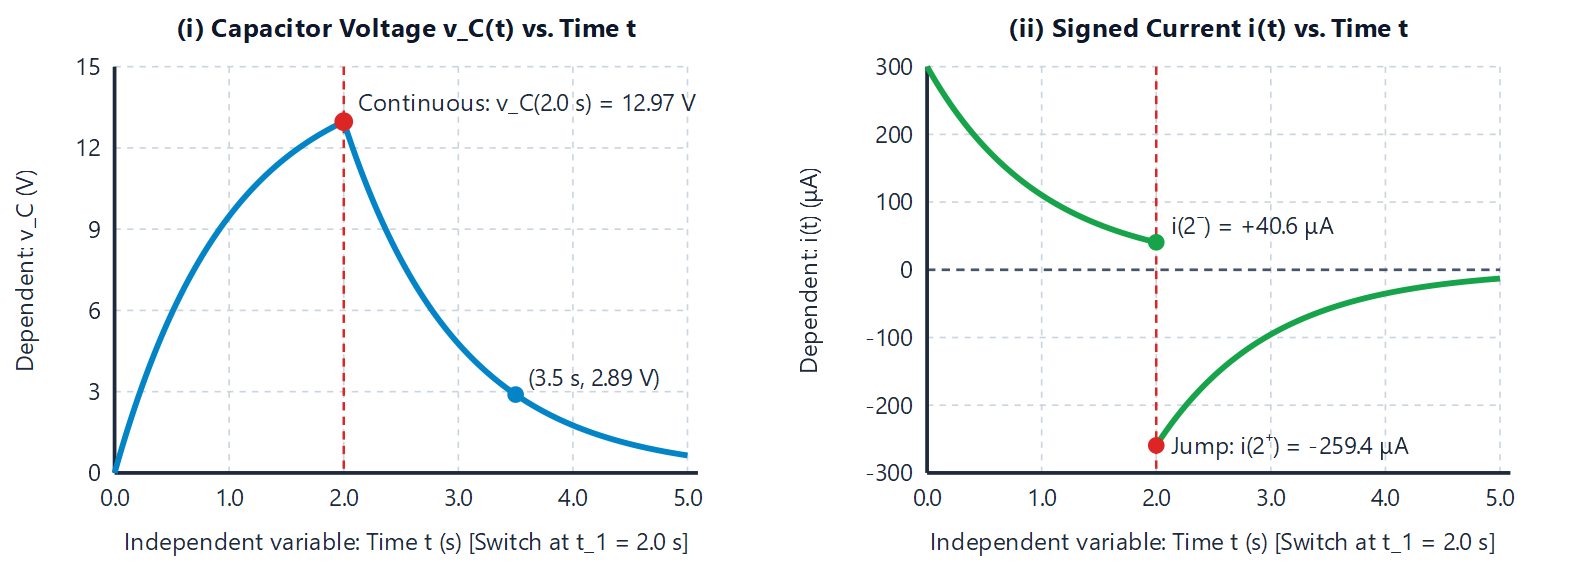
\includegraphics[width=0.82\linewidth]{day1_assets/s3-q4-grid-solved.png}\end{center}
\newpage
\section*{Block S4 Solutions: DC-Driven Series RLC Circuit Analysis}

  \textbf{Companion Key to:} \texttt{Block\_S4\_Exercises\_DC\_RLC\_Circuits.pdf} ~|~
  \textbf{Verification:} Cross-checked via Spec v2 MNA \& Exact 2nd-Order ODE Solver


\subsection*{01 $\cdot$ Solutions: Second-Order Series RLC ODE \& Critical Damping Proof \hfill [12 Points]}


  \subsubsection*{(a) Second-Order ODE in $v_C(t)$ [4 points]}
  By Kirchhoff's loop rule for $t \ge 0$, $\mathcal{E} - iR - L\frac{di}{dt} - v_C = 0 \implies L\frac{di}{dt} + Ri + v_C = \mathcal{E}$. Since $q = C v_C$, the series current and its derivative are $i = \frac{dq}{dt} = C\frac{dv_C}{dt}$ and $\frac{di}{dt} = C\frac{d^2 v_C}{dt^2}$. Substituting into KVL gives:
  $$LC\frac{d^2 v_C}{dt^2} + RC\frac{dv_C}{dt} + v_C = \mathcal{E} \quad \stackrel{\div LC}{\Longleftrightarrow} \quad \frac{d^2 v_C}{dt^2} + \frac{R}{L}\frac{dv_C}{dt} + \frac{1}{LC}v_C = \frac{\mathcal{E}}{LC}. \quad \blacksquare$$

  \subsubsection*{(b) Characteristic Equation, Roots \& $R_{\text{crit}} = 2\sqrt{L/C}$ [5 points]}
  Substituting $v_{C,h}(t) = A e^{st}$ into the homogeneous ODE yields $\left(s^2 + \frac{R}{L}s + \frac{1}{LC}\right)A e^{st} = 0$. By the quadratic formula:
  $$s_{1,2} = -\frac{R}{2L} \pm \sqrt{\left(\frac{R}{2L}\right)^2 - \frac{1}{LC}} = -\alpha \pm \sqrt{\alpha^2 - \omega_0^2}, \qquad \alpha = \frac{R}{2L}, \quad \omega_0 = \frac{1}{\sqrt{LC}}.$$
  Critical damping occurs when the two roots coalesce ($\alpha^2 - \omega_0^2 = 0$):
  $$\frac{R_{\text{crit}}}{2L} = \frac{1}{\sqrt{LC}} \implies R_{\text{crit}} = \frac{2L}{\sqrt{LC}} = 2\sqrt{\frac{L}{C}}. \quad \blacksquare$$

  \subsubsection*{(c) Underdamped Ringing Frequency $\omega'$ \& Assembled Step Response [3 points]}
  When $R < R_{\text{crit}}$, $\alpha < \omega_0$, so $\sqrt{\alpha^2 - \omega_0^2} = j\sqrt{\omega_0^2 - \alpha^2} = j\omega'$ where $\omega' = \sqrt{\frac{1}{LC} - \frac{R^2}{4L^2}}$. With particular solution $v_{C,p} = \mathcal{E}$, the general underdamped solution is $v_C(t) = \mathcal{E} + e^{-\alpha t}(C_1\cos\omega' t + C_2\sin\omega' t)$. Applying $v_C(0^+)=0 \implies C_1 = -\mathcal{E}$, and $\dot{v}_C(0^+) = -\alpha C_1 + \omega' C_2 = 0 \implies C_2 = -\frac{\alpha}{\omega'}\mathcal{E}$. Substituting $C_1$ and $C_2$ back assembles the complete underdamped step response:
  $$v_C(t) = \mathcal{E}\left[1 - e^{-\alpha t}\left(\cos(\omega' t) + \frac{\alpha}{\omega'}\sin(\omega' t)\right)\right]. \quad \blacksquare$$

Final Key (Ex 01): ~ $LC\ddot{v}_C + RC\dot{v}_C + v_C = \mathcal{E}$ ~|~ $R_{\text{crit}} = 2\sqrt{L/C}$, ~ $\omega' = \sqrt{\frac{1}{LC} - \frac{R^2}{4L^2}}$ ~|~ $v_C(t) = \mathcal{E}\left[1 - e^{-\alpha t}\left(\cos(\omega' t) + \frac{\alpha}{\omega'}\sin(\omega' t)\right)\right]$


\newpage



\subsection*{02 $\cdot$ Solutions: DC Step-Response Analysis ($V_s=12.0\text{ V}, R=40.0\ \Omega, L=0.800\text{ H}, C=500\ \mu\text{F}$) \hfill [14 Points]}


  \textbf{(a) Initial State at $t = 0^+$ [5 pts]:}
  \begin{itemize}
    \item By inductor current and capacitor voltage continuity: $i(0^+) = i(0^-) = 0\text{ A}$ and $v_C(0^+) = v_C(0^-) = 0\text{ V}$.
    \item Thus $v_R(0^+) = i(0^+) R = 0\text{ V}$, and by KVL at $t = 0^+$, the entire step voltage drops across the inductor: $v_L(0^+) = V_s - v_R(0^+) - v_C(0^+) = 12.0\text{ V}$.
    \item Initial derivatives: $\left.\dfrac{di}{dt}\right|_{0^+} = \dfrac{v_L(0^+)}{L} = \dfrac{12.0\text{ V}}{0.800\text{ H}} = 15.0\text{ A/s}$; $\left.\dfrac{dv_C}{dt}\right|_{0^+} = \dfrac{i(0^+)}{C} = 0\text{ V/s}$; $\left.\dfrac{d^2 v_C}{dt^2}\right|_{0^+} = \dfrac{1}{C}\left.\dfrac{di}{dt}\right|_{0^+} = \dfrac{15.0}{500\times 10^{-6}} = 3.00\times 10^4\text{ V/s}^2$.
  \end{itemize}
  \textbf{(b) DC Steady State ($t \to \infty$) \& Stored Energy [4 pts]:}
  \begin{itemize}
    \item As $t \to \infty$, $C$ acts as an \textbf{open circuit} and $L$ acts as a \textbf{short circuit}: $i(\infty) = 0\text{ A}$, $v_R(\infty) = 0\text{ V}$, $v_L(\infty) = 0\text{ V}$, and $v_C(\infty) = V_s = 12.0\text{ V}$.
    \item Stored energies: $U_L(\infty) = \frac{1}{2}L[i(\infty)]^2 = 0\text{ J}$, and $U_C(\infty) = \frac{1}{2}C[v_C(\infty)]^2 = \frac{1}{2}(500\times 10^{-6}\text{ F})(12.0\text{ V})^2 = 3.60\times 10^{-2}\text{ J} = 36.0\text{ mJ}$.
  \end{itemize}
  \textbf{(c) Damping Classification \& First Overshoot Peak [5 pts]:}
  $$\omega_0 = \frac{1}{\sqrt{(0.800)(500\times 10^{-6})}} = \frac{1}{\sqrt{4.00\times 10^{-4}}} = 50.0\text{ rad/s}, \qquad \alpha = \frac{R}{2L} = \frac{40.0}{2(0.800)} = 25.0\text{ s}^{-1},$$
  $$R_{\text{crit}} = 2\sqrt{\frac{L}{C}} = 2\sqrt{\frac{0.800}{500\times 10^{-6}}} = 2(40.0) = 80.0\ \Omega.$$
  Since $R = 40.0\ \Omega < R_{\text{crit}} = 80.0\ \Omega$ (or $\alpha = 25.0 < \omega_0 = 50.0$), the circuit is \textbf{underdamped} with ringing frequency:
  $$\omega' = \sqrt{50.0^2 - 25.0^2} = 25\sqrt{3} \approx 43.3\text{ rad/s}.$$
  Setting $\dot{v}_C(t) = \frac{V_s \omega_0^2}{\omega'} e^{-\alpha t}\sin(\omega' t) = 0$ gives the first peak at $t_{\text{peak}} = \frac{\pi}{\omega'} = \frac{\pi}{43.30} = 0.07255\text{ s} = 72.6\text{ ms}$, where:
  $$v_{C,\max} = 12.0\left(1 + e^{-\alpha \pi/\omega'}\right) = 12.0\left(1 + e^{-\pi/\sqrt{3}}\right) = 12.0(1 + 0.16303) = 13.96\text{ V} \approx 14.0\text{ V}.$$

Final Key (Ex 02): ~ $i(0^+)=0,\ v_C(0^+)=0,\ v_L(0^+)=12.0\text{ V},\ \dot{i}(0^+)=15.0\text{ A/s}$ ~|~ $v_C(\infty)=12.0\text{ V},\ U_C(\infty)=36.0\text{ mJ}$ ~|~ $R_{\text{crit}}=80.0\ \Omega$, Underdamped ($\omega'=43.3\text{ rad/s}$, peak $14.0\text{ V}$ at $72.6\text{ ms}$)

\subsection*{03 $\cdot$ Solutions: Step-Response Damping Curves \& Continuity Cloze \hfill [10 Points]}


  \textbf{Part B Cloze Key:} (a) \texttt{inductor current $i_L(t)$}, \texttt{inductor voltage $v_L(t)$}; (b) \texttt{open circuit}, \texttt{short circuit}; (c) \texttt{zero}; (d) \texttt{$2\sqrt{L/C}$}; (e) \texttt{underdamped}, \texttt{critically damped}.

\begin{center}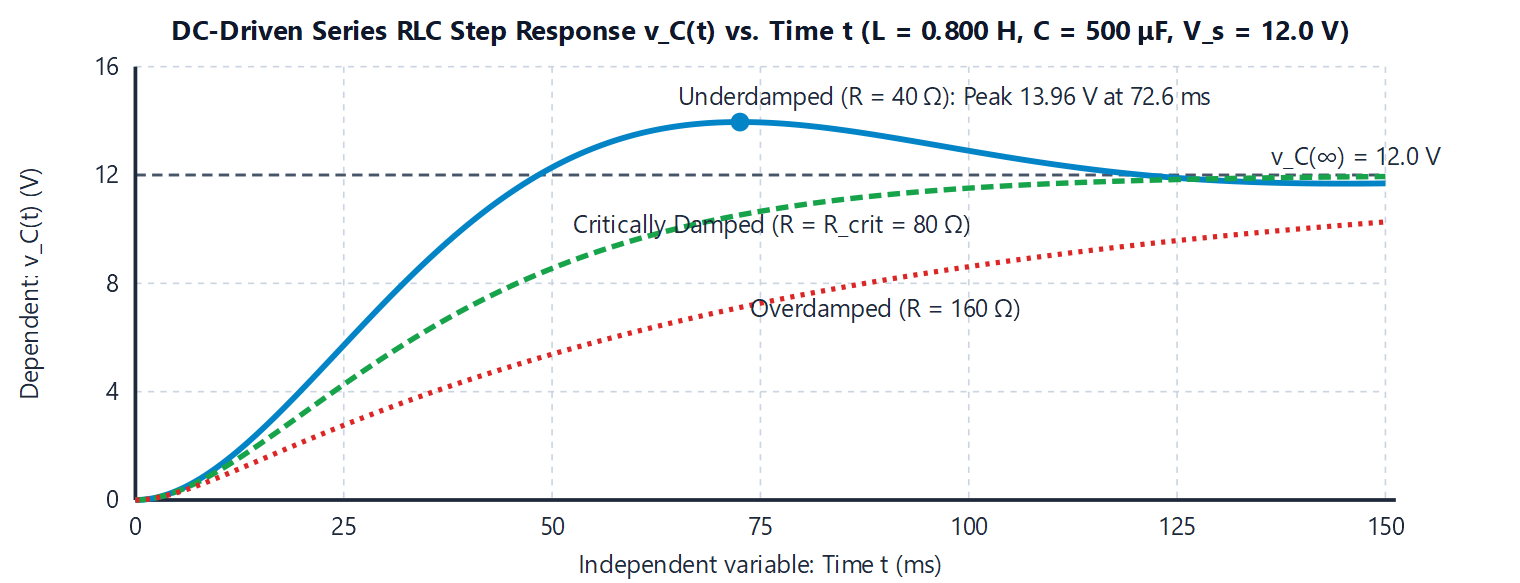
\includegraphics[width=0.82\linewidth]{day1_assets/s4-q3-grid-solved.png}\end{center}
\newpage
\section*{Block S5 Solutions: Series AC RLC Concepts, Inductance, Reactance \& Capacitance}

  \textbf{Companion Key to:} \texttt{Block\_S5\_Exercises\_AC\_RLC\_Reactance.pdf} ~|~
  \textbf{Verification:} Cross-checked via Spec v2 AC Phasor Solver


\subsection*{01 $\cdot$ Solutions: Reactance Proofs \& Solenoid Energy Density \hfill [12 Points]}


  \subsubsection*{(a) Differential Proofs of $X_L = \omega L$ and $X_C = \frac{1}{\omega C}$ [6 points]}
  \begin{itemize}
    \item \textbf{Inductor ($v_L = L\frac{di}{dt}$) [3 pts]:} With $i(t) = I_0\cos(\omega t)$:
    $$v_L(t) = L\frac{d}{dt}[I_0\cos(\omega t)] = -\omega L I_0 \sin(\omega t) = (\omega L I_0)\cos\left(\omega t + \frac{\pi}{2}\right) = V_{L,0}\cos\left(\omega t + \frac{\pi}{2}\right).$$
    Thus $V_{L,0} = I_0 X_L$ with $X_L = \omega L$, and $v_L(t)$ \textbf{leads} $i(t)$ by $+90^\circ$ ($+\pi/2\text{ rad}$).
    \item \textbf{Capacitor ($v_C = \frac{1}{C}\int i\,dt$) [3 pts]:} Integrating $i(t) = I_0\cos(\omega t)$:
    $$v_C(t) = \frac{1}{C}\int I_0\cos(\omega t)\,dt = \frac{I_0}{\omega C}\sin(\omega t) = \left(\frac{I_0}{\omega C}\right)\cos\left(\omega t - \frac{\pi}{2}\right) = V_{C,0}\cos\left(\omega t - \frac{\pi}{2}\right).$$
    Thus $V_{C,0} = I_0 X_C$ with $X_C = \dfrac{1}{\omega C}$, and $v_C(t)$ \textbf{lags} $i(t)$ by $-90^\circ$ ($-\pi/2\text{ rad}$).
  \end{itemize}

  \subsubsection*{(b) Solenoid Self-Inductance $L = \frac{\mu_0 N^2 A}{\ell}$ \& Energy Density $u_B = \frac{B^2}{2\mu_0}$ [6 points]}
  \begin{itemize}
    \item \textbf{Inductance [3 pts]:} Applying Amp\`ere's law $\oint \mathbf{B}\cdot d\mathbf{l} = \mu_0 I_{\text{enc}}$ to a rectangle of width $w$ enclosing $\frac{N}{\ell}w$ turns gives $B w = \mu_0 \left(\frac{N}{\ell}w\right)I \implies B = \frac{\mu_0 N I}{\ell}$. Flux through one turn is $\Phi_B = BA = \frac{\mu_0 N I A}{\ell}$, so total flux linkage is $N\Phi_B = \frac{\mu_0 N^2 A}{\ell}I = LI \implies L = \dfrac{\mu_0 N^2 A}{\ell}$.
    \item \textbf{Magnetic Energy \& Density [3 pts]:} $U_B = \int_0^I L i\,di = \frac{1}{2}LI^2 = \frac{1}{2}\left(\frac{\mu_0 N^2 A}{\ell}\right)I^2$. Dividing by the volume $V_{\text{vol}} = A\ell$ and substituting $I = \frac{B\ell}{\mu_0 N}$:
    $$u_B = \frac{U_B}{A\ell} = \frac{1}{2}\mu_0 \left(\frac{N I}{\ell}\right)^2 = \frac{1}{2}\mu_0 \left(\frac{B}{\mu_0}\right)^2 = \frac{B^2}{2\mu_0}. \quad \blacksquare$$
  \end{itemize}

Final Key (Ex 01): ~ $X_L = \omega L$ ($+90^\circ$ lead), $X_C = \frac{1}{\omega C}$ ($-90^\circ$ lag) ~|~ $L = \dfrac{\mu_0 N^2 A}{\ell}$, ~ $U_B = \frac{1}{2}LI^2$, ~ $u_B = \dfrac{B^2}{2\mu_0}$

\subsection*{02 $\cdot$ Solutions: 10-Blank Conceptual Cloze \& Resonance Self-Check \hfill [10 Points]}


  \textbf{Cloze Key (1 pt each = 10 pts; 4 unused distractors):} (a) \texttt{magnetic field}; (b) \texttt{in phase with}; (c) \texttt{leads}; (d) \texttt{lags}; (e) \texttt{open circuit ($X_C \to \infty$)}; (f) \texttt{$\sqrt{R^2 + (X_L - X_C)^2}$}; (g) \texttt{$1/\sqrt{LC}$}; (h) \texttt{minimum ($Z = R$)}; (i) \texttt{capacitive ($\phi < 0$)}; (j) \texttt{$\cos\phi = R/Z$}.
  \textbf{Self-Check Explanation:} At resonance, $v_L(t) = +V_{L,0}\cos(\omega_0 t + \pi/2)$ and $v_C(t) = +V_{C,0}\cos(\omega_0 t - \pi/2) = -v_L(t)$ are $180^\circ$ out of phase at every instant, so their instantaneous sum is $v_L(t) + v_C(t) = 0$ and KVL gives $v_s(t) = v_R(t)$ even when $V_{C,0} = V_{L,0} = \frac{X_C(\omega_0)}{R}V_0 = Q V_0 > V_0$ (for Exercise 03, $Q = \frac{100\ \Omega}{50.0\ \Omega} = 2.00$, so $V_{C,0} = V_{L,0} = 240\text{ V} = 2.00\,V_0$ while $V_0 = 120\text{ V}$).



\newpage



\subsection*{03 $\cdot$ Solutions: Series AC RLC Frequency Sweep ($V_0=120\text{ V}, R=50.0\ \Omega, L=0.200\text{ H}, C=20.0\ \mu\text{F}$) \hfill [12 Points]}


  \textbf{(a) Resonance ($\omega = \omega_0$) [4 pts]:}
  $$\omega_0 = \frac{1}{\sqrt{(0.200\text{ H})(20.0\times 10^{-6}\text{ F})}} = \frac{1}{\sqrt{4.00\times 10^{-6}}} = 500\text{ rad/s}, \qquad f_0 = \frac{500}{2\pi} = 79.6\text{ Hz}.$$
  At $\omega_0 = 500\text{ rad/s}$: $X_L = (500)(0.200) = 100\ \Omega$, $X_C = \frac{1}{(500)(20.0\times 10^{-6})} = 100\ \Omega$, $Z(\omega_0) = R = 50.0\ \Omega$, $I_0 = \frac{120\text{ V}}{50.0\ \Omega} = 2.40\text{ A}$, $\phi = 0^\circ$, $P_{\text{avg}} = \frac{1}{2}(2.40)^2(50.0) = 144\text{ W}$. Peak voltages: $V_{R,0} = (2.40)(50.0) = 120\text{ V}$, $V_{L,0} = V_{C,0} = (2.40)(100) = 240\text{ V} = 2.00\,V_0$ (they cancel in anti-phase!).

  \textbf{(b) Capacitive Regime ($\omega_1 = 250\text{ rad/s} = \frac{1}{2}\omega_0$) [4 pts]:}
  $$X_L(\omega_1) = (250)(0.200) = 50.0\ \Omega, \quad X_C(\omega_1) = \frac{1}{(250)(20.0\times 10^{-6})} = 200\ \Omega, \quad X = 50.0 - 200 = -150\ \Omega.$$
  $$Z(\omega_1) = \sqrt{50.0^2 + (-150)^2} = 50\sqrt{10} \approx 158\ \Omega, \quad I_0(\omega_1) = \frac{120}{50\sqrt{10}} = 0.759\text{ A}, \quad \phi_1 = \arctan(-3.00) = -71.6^\circ.$$
  Power factor $\cos\phi_1 = \frac{R}{Z} = \frac{1}{\sqrt{10}} = 0.316$, $P_{\text{avg}}(\omega_1) = \frac{1}{2}I_0^2 R = 14.4\text{ W}$, and $i(t) = (0.759\text{ A})\cos(250 t + 1.25\text{ rad})$.

  \textbf{(c) Inductive Regime ($\omega_2 = 1000\text{ rad/s} = 2\omega_0$) [4 pts]:}
  $$X_L(\omega_2) = (1000)(0.200) = 200\ \Omega, \quad X_C(\omega_2) = \frac{1}{(1000)(20.0\times 10^{-6})} = 50.0\ \Omega, \quad X = +150\ \Omega.$$
  $$Z(\omega_2) = 50\sqrt{10} \approx 158\ \Omega, \quad I_0(\omega_2) = 0.759\text{ A}, \quad \phi_2 = +71.6^\circ, \quad P_{\text{avg}}(\omega_2) = 14.4\text{ W}.$$
  Because $\omega_1 \omega_2 = \omega_0^2$, $X_L(\omega_2) = X_C(\omega_1)$ and $X_C(\omega_2) = X_L(\omega_1)$, so $|X_L - X_C|$ is identical while $(X_L - X_C)$ flips sign!

Final Key (Ex 03): ~ $\omega_0 = 500\text{ rad/s},\ Z_{\min}=50.0\ \Omega,\ I_{0,\max}=2.40\text{ A},\ P_{\max}=144\text{ W}$ ~|~ At $\omega_1=250,\ \omega_2=1000\text{ rad/s}$: $Z=158\ \Omega,\ I_0=0.759\text{ A},\ \phi=\mp 71.6^\circ,\ P_{\text{avg}}=14.4\text{ W}$

\subsection*{04 $\cdot$ Solutions: Frequency-Response Graphs \& Phasor Diagrams \hfill [10 Points]}
\begin{center}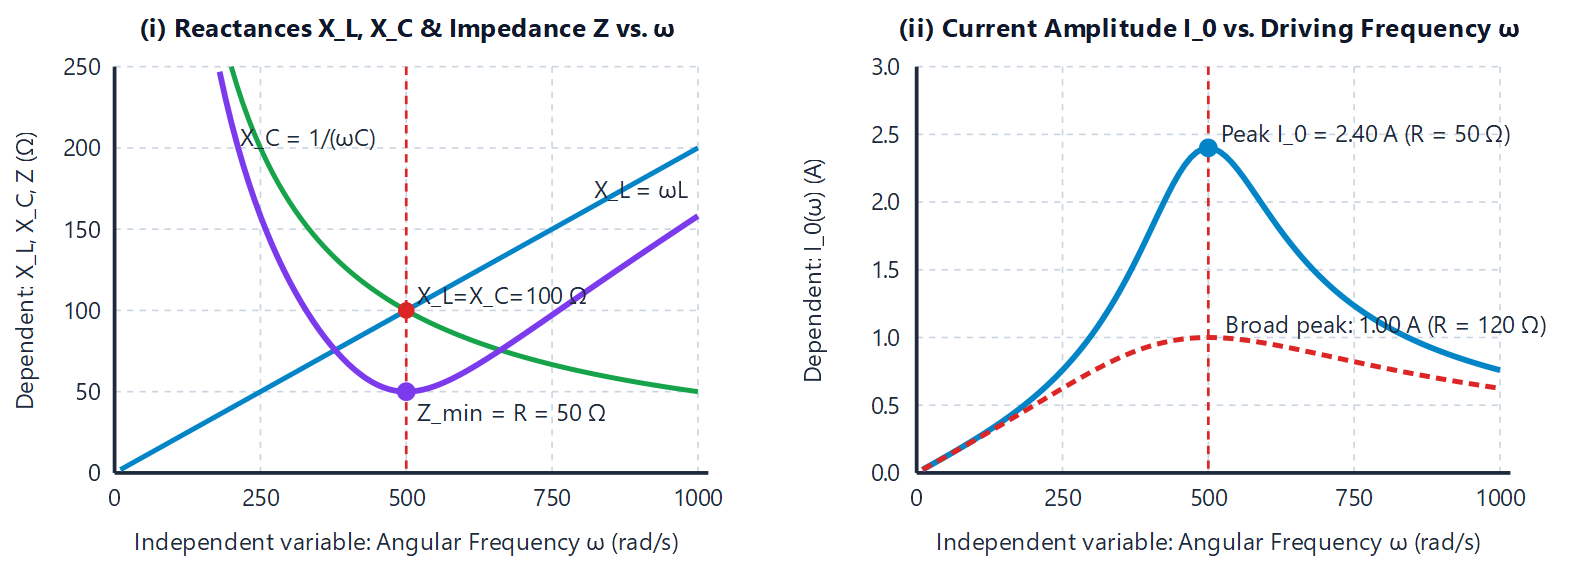
\includegraphics[width=0.82\linewidth]{day1_assets/s5-q4-grid-solved.png}\end{center}
\begin{center}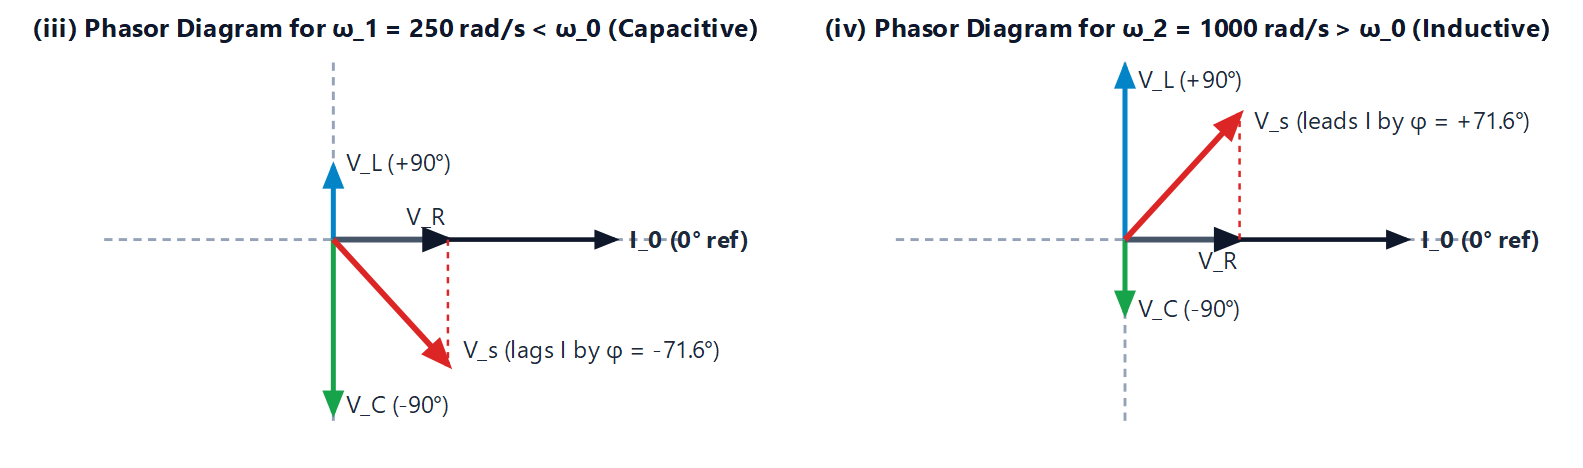
\includegraphics[width=0.82\linewidth]{day1_assets/s5-q4-phasors-solved.png}\end{center}

\end{document}
